% Options for packages loaded elsewhere
\PassOptionsToPackage{unicode}{hyperref}
\PassOptionsToPackage{hyphens}{url}
%
\documentclass[
]{article}
\usepackage{lmodern}
\usepackage{amssymb,amsmath}
\usepackage{ifxetex,ifluatex}
\ifnum 0\ifxetex 1\fi\ifluatex 1\fi=0 % if pdftex
  \usepackage[T1]{fontenc}
  \usepackage[utf8]{inputenc}
  \usepackage{textcomp} % provide euro and other symbols
\else % if luatex or xetex
  \usepackage{unicode-math}
  \defaultfontfeatures{Scale=MatchLowercase}
  \defaultfontfeatures[\rmfamily]{Ligatures=TeX,Scale=1}
\fi
% Use upquote if available, for straight quotes in verbatim environments
\IfFileExists{upquote.sty}{\usepackage{upquote}}{}
\IfFileExists{microtype.sty}{% use microtype if available
  \usepackage[]{microtype}
  \UseMicrotypeSet[protrusion]{basicmath} % disable protrusion for tt fonts
}{}
\makeatletter
\@ifundefined{KOMAClassName}{% if non-KOMA class
  \IfFileExists{parskip.sty}{%
    \usepackage{parskip}
  }{% else
    \setlength{\parindent}{0pt}
    \setlength{\parskip}{6pt plus 2pt minus 1pt}}
}{% if KOMA class
  \KOMAoptions{parskip=half}}
\makeatother
\usepackage{xcolor}
\IfFileExists{xurl.sty}{\usepackage{xurl}}{} % add URL line breaks if available
\IfFileExists{bookmark.sty}{\usepackage{bookmark}}{\usepackage{hyperref}}
\hypersetup{
  hidelinks,
  pdfcreator={LaTeX via pandoc}}
\urlstyle{same} % disable monospaced font for URLs
\usepackage{graphicx,grffile}
\makeatletter
\def\maxwidth{\ifdim\Gin@nat@width>\linewidth\linewidth\else\Gin@nat@width\fi}
\def\maxheight{\ifdim\Gin@nat@height>\textheight\textheight\else\Gin@nat@height\fi}
\makeatother
% Scale images if necessary, so that they will not overflow the page
% margins by default, and it is still possible to overwrite the defaults
% using explicit options in \includegraphics[width, height, ...]{}
\setkeys{Gin}{width=\maxwidth,height=\maxheight,keepaspectratio}
% Set default figure placement to htbp
\makeatletter
\def\fps@figure{htbp}
\makeatother
\setlength{\emergencystretch}{3em} % prevent overfull lines
\providecommand{\tightlist}{%
  \setlength{\itemsep}{0pt}\setlength{\parskip}{0pt}}
\setcounter{secnumdepth}{-\maxdimen} % remove section numbering

\date{}

\documentclass[11pt]{article} 
\begin{document}

\title{Assignment 5}
\author{Raymond Baker}
\date{\today}

\includegraphics[width=\columnwidth]{ryerson_logo.png}

\begin{flushleft}
\begin{tabular}{|p{0.4\textwidth}|p{0.6\textwidth}|} 
 \hline
    Course Title: & Digital Image Processing \\ [5ex]
 \hline
    Course Number: & ELE 882 \\ [5ex]
 \hline
    Semester/Year & Fall/2019 \\ [5ex]
 \hline

\end{tabular}
\end{flushleft}

\begin{flushleft}
\begin{tabular}{|p{0.4\textwidth}|p{0.6\textwidth}|} 
 \hline
    Instructor: & Ling Guan \\ [5ex]
 \hline
\end{tabular}
\end{flushleft}

\begin{flushleft}
\begin{tabular}{|p{0.4\textwidth}|p{0.6\textwidth}|} 
 \hline
    Assignment/Lab Number: & 5 \\[5ex]
 \hline
    Assignment/Lab Title: & Assignment 5 \\[5ex]
 \hline
\end{tabular}
\end{flushleft}

\begin{flushleft}
\begin{tabular}{|p{0.4\textwidth}|p{0.6\textwidth}|} 
 \hline
    Submission Date: & \today \\[5ex]
 \hline
    Due Date: & \today \\[5ex]
 \hline
\end{tabular}
\end{flushleft}

\begin{flushleft}
\begin{tabular}{|p{0.2\textwidth}|p{0.2\textwidth}|p{0.22\textwidth}|p{0.09\textwidth}|p{0.19\textwidth}|}
 \hline
     Student \linebreak LAST Name & Student \linebreak FIRST Name & Student \linebreak Number & Section & Signature* \\
 \hline
    Baker & Raymond & 500691429 & 03 & R.B. \\[5ex]
 \hline
    Bao & Doan & 500733516 & 03 & B.D. \\[5ex]
 \hline
\end{tabular}
\end{flushleft}

\pagebreak
\textbf{3.1.1 RGB to HSI}
\begin{verbatim}
function out = rgb_to_hsi(img)
img=double(img)/255;

R=img(:,:,1);
G=img(:,:,2);
B=img(:,:,3);

numi=1/2*((R-G)+(R-B));
denom=((R-G).^2+((R-B).*(G-B))).^0.5;

H=acos(numi./(denom));
H(R==0 & G==0 & B==0) = 0;
H(B>G)=2*pi-H(B>G);

cmin = min(img, [], 3);
S=1- (3./(sum(img,3)+0.000001)).*cmin;

I=sum(img,3)./3;
out=cat(3,H,S,I);
end
\end{verbatim}
\pagebreak

\textbf{3.1.2 HSI to RGB}
\begin{verbatim}
function out = hsi_to_rgb(img)
   
    img = double(img);
    length = size(img, 1);
    width = size(img, 2);
    
    r = zeros(length, width);
    g = zeros(length, width);
    b = zeros(length, width);
   
   for i=1:(length) 
         for j=1:(width)
            H= (img(i,j,1));
            S= (img(i,j,2));
            I= (img(i,j,3));
            if ( 0<=H && H<((2/3)*pi))
                r(i,j) = I*(1+(S*cos(H))/cos((pi/3)-H));
                b(i,j) = I*(1-S);
                g(i,j) = 3*I -(r(i,j)+b(i,j));
            elseif ( ((2/3)*pi)<=H && H<((4/3)*pi))
                H=H-((2/3)*pi);
                r(i,j) = I*(1-S);
                g(i,j) = I*(1+(S*cos(H))/cos((pi/3)-H));
                b(i,j) = 3*I -(r(i,j)+g(i,j));
            elseif ( ((4/3)*pi)<=H && H<=(2*pi))
                H=H-((4/3)*pi);
                g(i,j) = I*(1-S);
                b(i,j) = I*(1+(S*cos(H))/cos((pi/3)-H));
                r(i,j) = 3*I -(g(i,j)+b(i,j));     
            end    
         end 
     end    
    
    
    out = cat(3, r, g, b);
    
end

\end{verbatim}
\includegraphics[width=1\columnwidth]{RGB Pic.png}

\pagebreak

\textbf{3.1.3 RGB to YCBCR}
\begin{verbatim}
function out = rgb_to_ycbcr(img)
    r = double(img(:,:,1));
    g = double(img(:,:,2));
    b = double(img(:,:,3));

    h = [[0.299,0.587,0.114];
        [-0.1687,-0.3313,0.5];
        [.5, -0.4187, -0.0813]];
    
    length = size(img, 1);
    width = size(img, 2);
    
    out = img;
    
    %If b <= g
    for x = 1:length
        for y = 1:width
            temp = h*([r(x,y), g(x,y), b(x,y)]');
            y(x, y) = temp(1);
            cb (x, y) = temp(2) + 128;
            cr(x, y) = temp(3) + 128;
        end
    end
    
    out = cat(3, yc, b, cr);
end
\end{verbatim}

\pagebreak

\textbf{3.1.4 YCBCR to RGB}
\begin{verbatim}
function out = ycbcr_to_rgb(img)
    r = double(img(:,:,1));
    g = double(img(:,:,2));
    b = double(img(:,:,3));

    h = [[1,0,1.402];
        [1,-0.34414,-0.71414];
        [1,1.772,0]];
    
    length = size(img, 1);
    width = size(img, 2);
    
    out = img;
    
    %If b <= g
    for x = 1:length
        for y = 1:width
            temp = h*([r(x,y), g(x,y) - 128, b(x,y) - 128]');
            yc(x, y) = temp(1);
            b (x, y) = temp(2);
            cr(x, y) = temp(3);
        end
    end
    
    out = uint8(cat(3, yc, b, cr));
end
\end{verbatim}

\pagebreak

\includegraphics[width=1\columnwidth]{ycbcr.png}

\pagebreak

\textbf{3.2.1 Change Hue}
\begin{verbatim}
function out = change_hue(img, angle) 
    out = img;
    out(:,:,1) = mod(out(:,:,1) + angle, 2*pi);
end

figure(3);
imshow(hsi_to_rgb(change_hue(rgb_to_hsi(a), 2/3*pi)));
\end{verbatim}

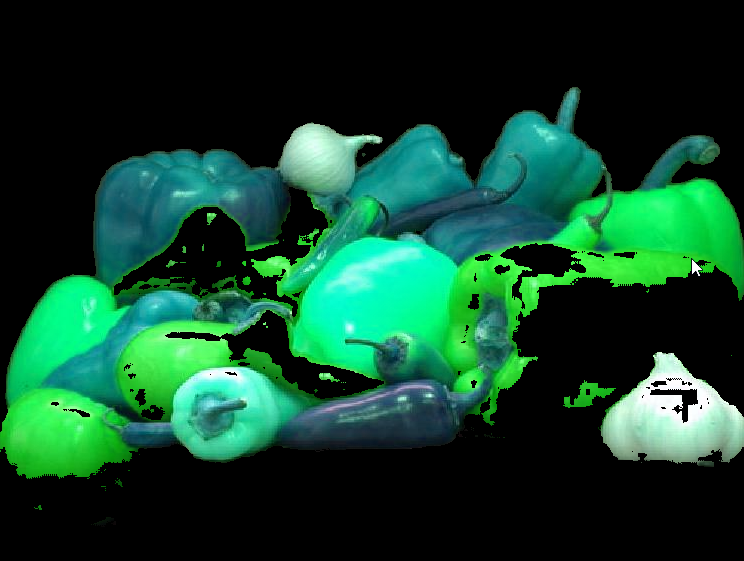
\includegraphics[width=0.5\columnwidth]{Change Hue.png}

\pagebreak

\textbf{3.2.2 Change Saturation}
\begin{verbatim}
function out = change_saturation(img, sat_off) 
    out = img;
    sat = out(:,:,2);    
    
    sat = sat + sat_off;
    sat(sat>1) = 1;
    
    out(:,:,2) = sat;
end

figure(4);
imshow(hsi_to_rgb(change_saturation(rgb_to_hsi(a), 0.2)));
\end{verbatim}

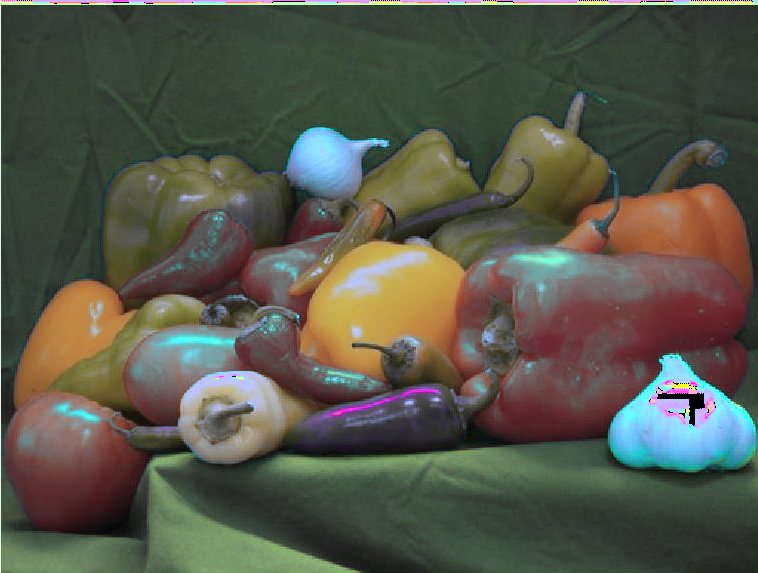
\includegraphics[width=0.5\columnwidth]{Change Sat.png}

\pagebreak


\textbf{3.2.3 Apply Point Trfm}
\begin{verbatim}
function output_img = apply_point_trfm (input_img, b, c)
    output_img = (double(input_img) * b) + c;
    output_img = uint8(output_img);
end

bright = apply_point_trfm(a, 2, 10);
figure(5);
imshow(bright);
\end{verbatim}

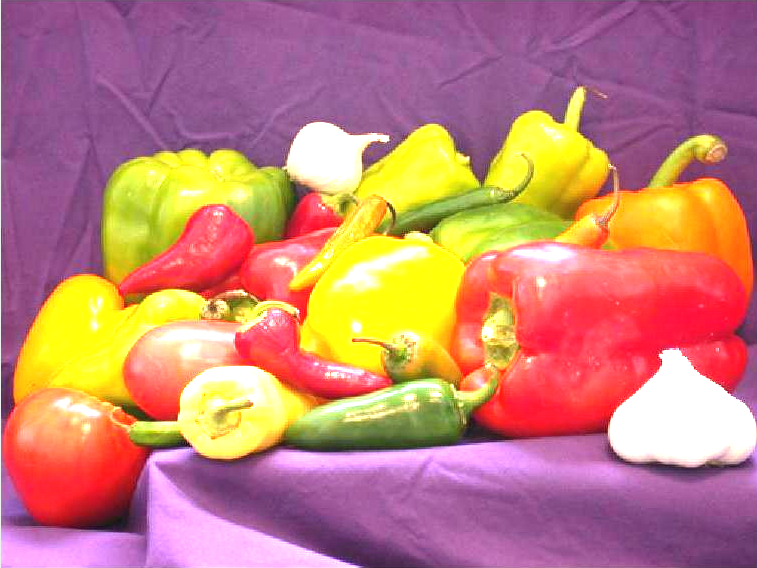
\includegraphics[width=0.5\columnwidth]{Point Trfm.png}

\pagebreak
\textbf{3.2.4 Spatial Filter}
\begin{verbatim}
function output = spatial_filter (img, h)
    w = size(h, 1);
    h_ = size(h, 2);
    new_h = (h_-1)/2;
    new_w = (w-1)/2;
    padded = padarray(img, [new_w, new_h], 'both');
    output = img;
    for x = (1:size(img, 1))
        for y =(1:size(img, 2))
            output(x, y, 1) = sum(sum(double(padded(x:x+w-1, y:y+h_-1, 1)).* h));
            output(x, y, 2) = sum(sum(double(padded(x:x+w-1, y:y+h_-1, 2)).* h));
            output(x, y, 3) = sum(sum(double(padded(x:x+w-1, y:y+h_-1, 3)).* h));
        end
    end
end

figure(6);
imshow(spatial_filter(a, [[0,1,1];[-1,1,1];[-1,-1,0]]));
\end{verbatim}

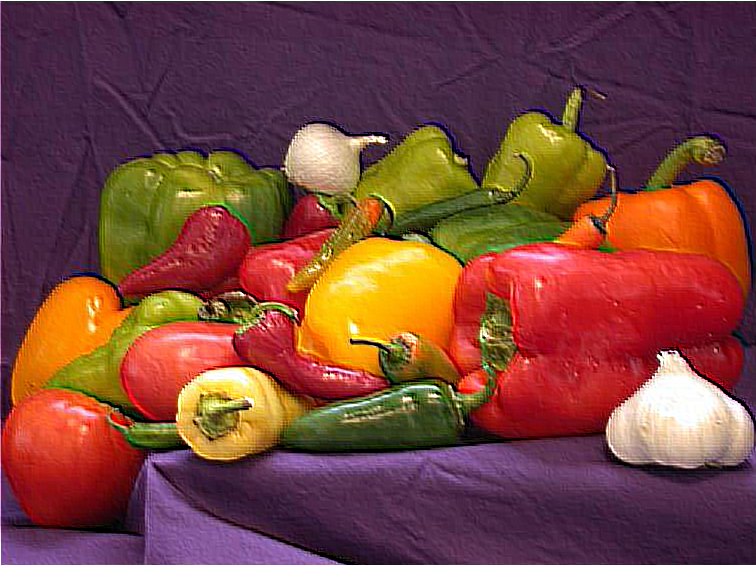
\includegraphics[width=0.5\columnwidth]{Spatial Filter.png}

\pagebreak
\textbf{3.2.5 Histogram Equalize RGB}
\begin{verbatim}
function out = histogram_equalize(img)
    total_count = size(img, 1) * size(img, 2);
    
    r = img(:,:,1);
    g = img(:,:,2);
    b = img(:,:,3);
    
    for i = 0:255
        new_val = floor(length(r(r <= i))/total_count*255);
        r(r==i) = new_val;
        new_val = floor(length(g(g <= i))/total_count*255);
        g(g==i) = new_val;
        new_val = floor(length(b(b <= i))/total_count*255);
        b(b==i) = new_val;
    end
    out = cat(3, r, g, b);
end

figure(7);
imshow(histogram_equalize(a));

\end{verbatim}

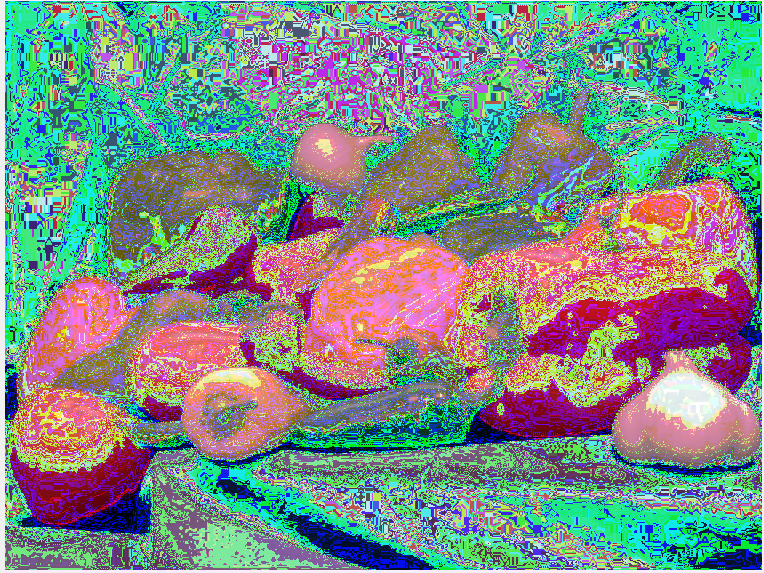
\includegraphics[width=0.5\columnwidth]{Hist Eq RGB.png}

\pagebreak
\textbf{3.2.5 Histogram Equalize YCBCR}
\begin{verbatim}
function out = histogram_equalize_ycbcr(img)
    total_count = size(img, 1) * size(img, 2);
    
    ycbcr_img = rgb_to_ycbcr(img);
    
    y = ycbcr_img(:,:,1);
    for i = 0:255
        new_val = floor(length(y(y <= i))/total_count*255);
        y(y==i) = new_val;
    end
    
    ycbcr_img(:,:,1) = y;
    
    out = ycbcr_to_rgb(ycbcr_img);
end

figure(8);
imshow(histogram_equalize_ycbcr(a));

\end{verbatim}

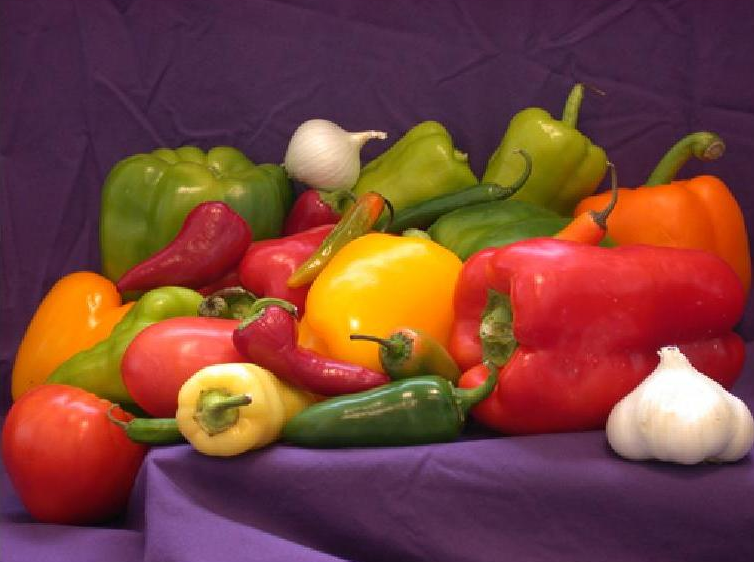
\includegraphics[width=0.5\columnwidth]{YCBCR Hist Eq.png}



\pagebreak
\textbf Analysis

\textbf {Q1. For histogram equalization, is there any difference between applying the operation to
each colour channel separately or by first performing a colour conversion, histogram equalizing
the luma channel and then going back to RGB? Are the results better or worse? Explain why or
why not. Ignore any performance considerations.}

There is a difference between applying histogram equalization on each RGB channel separately verses just the luma. The results are better when doing histogram equalization on the luma channel, because it only equalizes the brightness. While  RGB histogram equalization applies to each colour separately resulting in artifacts.

\textbf{Q2. Is any reason why we would prefer to process in the Y’CbCr space over the HSI for the
colour-based histogram equalization?}

When converting between RGB and Y'CbCr colour space, it is less computationally expensive when compared to the HSI colour space. The conversion between RGB and Y'CbCr is done through a matrix multiplication, both to and from the Y'CbCr colour space. In comparison, HSI requires the calculation of three values, the angle (H), saturation value (S) and intensity values (I). 


\textbf{Q3. Conversely, why would we prefer to use the HSI space over the Y’CbCr space when
modifying the colour properties of an image?}

HSI is useful for changing colour properties because the encoding directly maps to useful properties for manipulation. Hue represents the colour, Saturation represents the intensity of that colour and Intensity represents the brightness of the colour. On the contrary YCbCr encodes the image in less useful properties for manipulation. Y(luma) represents the brightness of the colour, Cb represents blue difference and Cr represents red difference.

\textbf{Q4. How would you modify the edge detector from Assignment 2 to handle colour information? Consider the fact an edge in a colour image may disappear when converted to greyscale.}

To implement an edge detector on a color image, one can apply the vertical and horizontal gradient of each channel separately and add them together. With the resulting images find the magnitude. 

\end{document}
